\section{Dynamics\label{dynamics}}

The I/O automata model assumes that systems are composed of a finite or infinitely countable number of automata~\cite{lynch1996distributed}.
Assuming an infinitely countable number of participants allows properties of the systems to be stated in terms of an abstract quantity representing the number of members, e.g., $N$, and is reasonable because all real systems are composed of a finite number of members.
The set of interactions in the I/O automata model is also fixed since automata are statically composed.
Dynamic systems are modeled by assuming that only a subset of the all the automata that could possibly exist are actively participating in the system.
To use this technique, a flag is associated with each automaton indicating if it is active or inactive and external actions for ``waking up'' and ``going to sleep'' are defined~\cite{lynch1996distributed}.

While assuming a fixed number of automata is reasonable for modeling, assuming a fixed number of automata for a real system results in over-provisioning or inflexibility.
To develop a component based on the static I/O automata model, a developer must choose a concrete value for the abstract quantity $N$.
System resources are wasted if the actual number of participants is much smaller than $N$.
If the number of participants is greater than $N$, then the system cannot respond to certain situations even though resources might be available.
Consequently, a system built using the component model described in section~\ref{system_model} requires the ability to deal with a dynamic set of automata and interactions.

\paragraph{System actions.}
The four indivisible operations for managing a dynamic set of automata are create, bind, unbind, and destroy.
Create, bind, unbind, and destroy are collectively called \emph{system actions}.
The \emph{create} operation allows an automaton to create a child automaton.
The \emph{bind} operation allows an automaton to bind an input action to an output action while the \emph{unbind} operation allows an automaton to separate an input action from an output action.
The \emph{destroy} operation allows an automaton to recursively destroy a child automaton and all bindings associated with it.

System actions can fail for a variety of reasons.
A create fails if the automaton that should be added to the set of automata, i.e., the automata being created, already exists.
A bind fails if the automaton associated with the output action doesn't exist, the automaton associated with the input action doesn't exist, or any of the binding rules outlined in section~\ref{system_model} would be violated.
An unbind fails if the binding does not exist.
Note that the owner of binding is taken into account when determining if the binding exist so only the owner of a binding can dissolve it.
A destroy fails if the automaton being destroyed does not exist or is not a child of the automaton requesting the destroy.

%% Let $A$ be the set of automata that exist where each element in $A$ is a pair $(p, a)$ where $p$ is the parent of $a$.
%% Let $B$ be the set of bindings that exist where each element in $B$ is a tuple $(w, o_a, o_n, o_p, i_a, i_n, i_p)$ where $w$ is the automaton that owns the binding, $o_a$ is the output automaton, $o_n$ is the name of the output action, $o_p$ is the parameter of the output action, $i_a$ is the input automaton, $i_n$ is the name of the input action, and $i_p$ is the parameter of the input action.
%% Define the predicate $exists (a) = \langle \exists p, q : (p, q) \in A :: q = a\rangle$ that is true when automaton $a$ exists, i.e., has a parent\footnote{The root automaton's parent is the special symbol $\perp$.}.
%% Define the predicate $existsb (a) = \langle \exists a : (w, o_a, o_n, o_p, i_a, i_n, i_p) \in B :: a = w \lor a = o_a \lor a = i_a \rangle$ that is true when automaton $a$ appears somewhere in $B$.
%% We define the create operation as the Hoare triple $\{exists (p) \land \lnot exists (a)\} \quad create(a)_p \quad \{(p,a) \in A\}$ which says that the parent automaton $p$ can create automaton $a$ if $p$ exists and $a$ does not exist.
%% The destroy operation can be defined $\{(p,a) \in A\} \quad destroy(a)_p \quad \{(p,a) \notin A \land \lnot existsb(a)\}$ which says that in order to destroy $a$ and remove all bindings associated with $a$, $p$ must be the parent of $a$.
%% Define the predicate $free (a, n, p) = \langle \forall w, o_a, o_n, o_p, i_a, i_n, i_p : (w, o_a, o_n, o_p, i_a, i_n, i_p) \in B :: \lnot (i_a = a \land i_n = n \land i_p = p) \rangle$ that is true when the input action argument is not bound.
%% Define the predicate $involved (o, n, p, i) = \langle \exists w, o_a, o_n, o_p, i_a, i_n, i_p : (w, o_a, o_n, o_p, i_a, i_n, i_p) \in B :: o_a = o \land o_n = n \land o_p = p \land i_a = i \rangle$ that is true when automaton $o$'s output action $(n, p, i)$ is bound to some input action in automaton $i$.
%% The bind operation can be defined $\{exists (w) \land exists (o_a) \land exists (i_a) \land free (i_a, i_n, i_p) \land \lnot involved(o_a, o_n, o_p, i_a) \land o_a \neq i_a \} \quad bind (w, o_a, o_n, o_p, i_a, i_n, i_p) \quad \{(w, o_a, o_n, o_p, i_a, i_n, i_p) \in B\}$ which says that in order for the binding to succeed the owner $w$ exists, automaton $o_a$ exists, automaton $i_a$ exists, the input action $(i_a, i_n, i_p)$ must not be bound, the output action $(o_n, o_p)$ of automaton $o_a$ cannot be bound to an input action in automaton $i_a$, and the automata $o_a$ and $i_a$ cannot be the same.
%% The precondition for $bind$ is same as the binding rules derived in section~\ref{system_model} augmented with existence tests for the owner, output automaton, and input automaton.
%% The unbind operation is similar to destroy: $\{(w, o_a, o_n, o_p, i_a, i_n, i_p) \in B\} \quad unbind (w, o_a, o_n, o_p, i_a, i_n, i_p) \quad \{(w, o_a, o_n, o_p, i_a, i_n, i_p) \notin B\}$.

% I didn't do more complex transactions, i.e., create-and-bind, because its not clear how it fails.
% Are partial successes allowed?
% Furthermore, such  transactions can be arbitrarily complex which doesn't bode well for efficiency.

\begin{figure}
\center
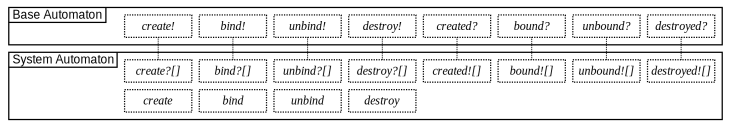
\includegraphics[width=\textwidth]{system_action}
\caption{System actions.
  An automaton contains output actions for creating, binding, unbinding, and destroying.
  The system automaton contains parameterized input actions for receiving the requests to create, binding, unbind, and destroy.
  The system automaton returns a result using the appropriate parameterized output action.
  The automaton contains input actions to receive the results.}
\label{system_action}
\end{figure}

\paragraph{The system automaton.}
Let the set of automata $A$ and set of bindings $B$ be managed by the \emph{system automaton} which represents the run-time system.
Each automaton is composed (not bound) with the system automaton and has output actions for requesting system actions and input actions for receiving the results of system actions.
The system automaton, in turn, has input actions for receiving requests for system actions, possibly some internal actions for evaluating system action requests, and output actions for responding with the result of system actions.
Figure~\ref{system_action} shows the relationship between an automaton and the system automaton.

Conceptually, the state variables $A$ and $B$ belong to the system automaton.
However, the state encoded by $A$ and $B$ is shared and used in the execution of every action.
The scheduler uses $A$ to ensure that only actions belonging to automata exist are selected and uses $B$ to ensure that the appropriate set of inputs actions receive the value produced when an output action is executed.
Thus, the set of actions implied by any action is the set defined in section~\ref{system_model} \emph{and} and the system automaton.
However, the opportunities for concurrency explored in section~\ref{system_model} are not lost when one considers that the only actions that modify $A$ and $B$ must be serialized, i.e., not executed concurrently with other actions.

\paragraph{Binding predicates.}
The static configuration of a system as prescribed by the I/O automata model guarantees that the set of implied automata for an action is always the same.
This property is necessary and desirable for reasoning about the behavior of the system.
Admitting dynamics removes this guarantee since the set of implied automata will change according to the various system actions being executed.
To be specific, the set of implied automata for internal actions does not change but the set of implied automata for output actions can be changed with a successful bind, unbind, or destroy.

To force a dynamic system to behave like a static system, the execution of output actions must be delayed until the set of implied automata matches the set implied by the static system.
To do this, we conjunct the precondition of an output action with a predicate over the set of bindings $B$ to ensure that the output action is not executed until its set of implied automata is correct.
Notice that this only requires reading $B$ and is permitted based on the required properties of the system automaton.
Thus, a dynamic system can be analyzed as a static system by ignoring system actions and the binding predicates.
A static system can be implemented by adding binding predicates and logic to create the constellation of automata.

%% All components have outputs for creating, binding, unbinding, and destroying and inputs for receiving results that are permanently bound to ``the system.''
%% System calls follow a request-reply system where a component sends a request for a create, bind, unbind, or destroy, the system receives the request, the system processes the request, the system sends a reply, and the component receives the reply.

%Events can be bound and unbound at run-time.
%% The I/O automata model is static, i.e., the set of automata and their interactions are fixed.
% Components can be created and destroyed at run-time.


%% \subsection{I/O Automata and Dynamic Configuration}

%% A standard technique for modeling dynamic modules in I/O automata is to assume they exist but are inactive.
%% Dynamic automata can then be activated and deactivated using inputs.
%% We will use a similar technique to model dynamic configurations.

%% We introduce a \emph{system automaton} that records the configuration of all automata in the system.
%% We differentiate between automaton types and automaton instances.
%% Every automaton instances has a unique \emph{automaton identifier (aid)}.
%% The state of the system automaton consists of the set of aids $A$ indicating what automata exist and a set of binding records $B$ indicating the relationship between output and input actions.
%% A binding record $(out, output, in, input)$ is tuple consisting of the aid of the output automaton $out$, the name of the output action $output$, the aid of the input automaton $in$, and the name of the input action $input$.

%% The configuration contained in set of binding records must be a valid static configuration to ensure that the behavior of the complete system remains analyzable under the I/O automata model.
%% First, the output automaton and input automaton must exist $\forall (out, output, in, input) \in B: out \in A \land in \in A$.
%% % TODO:  Binding must not exist.
%% Second, an input can only be bound to one output.
%% Thus, a given $in$ and $input$ combination can appear at most once in $B$.
%% Third, an output cannot be bound to an input in the same automaton.
%% Thus, $out \neq in$ for every $(out, output, in, input)$ in $B$.
%% Fourth, an output cannot be bound to two inputs in the same automaton.
%% Thus, $in_1 \neq in_2$ for all $(out, output, in_1, input_1), (out, output, in_2, input_2)$ in $B$.

%% The system automaton contains input actions for creating an automaton, binding an output to an input, unbinding an output and an input, and destroying an automaton and output actions that indicate the result of a create, bind, unbind, or destroy.
%% All automata are composed with the system automaton and contain outputs for creating, binding, unbinding, and destroying and inputs for receiving results.
%% Systems calls (create, bind, unbind, destroy) resemble a request-response protocol where an automaton sends a request, the system automaton receives the request, the system processes the request, the system automaton then sends the result, and the automaton receives the result.
%% This has the important consequence that \emph{configuration is asynchronous}.
%% Destroying an automaton has the effect of removing all of its bindings.
%% An automaton that destroys itself can therefore cause the system to deliver unbound and destroyed events without an unbind or destroy.

%% Using the system automaton as a bookkeeping mechanism, we can relate a statically composed system to a dynamically configured one.
%% The key idea is to show that actions belong to automaton $a$ are only executed when $a \in A$ and that an output action is only executed when $B$ contains all of bindings associated with the static configuration.


%% \subsection{Extending I/O Automata for Reflection}

%% Automata are endowed with additional inputs driven by system outputs indicating when an action has been bound and unbound.
%% Automata might use the bound input to enable processing, i.e., someone is listening so I'll start producing data.
%% The unbound input is useful for cleaning data structures and inhibiting further processing, i.e., no one is listening so I'll stop producing data.
%% The bound and unbound inputs are useful but they are also asynchronous, thus, an automaton cannot trust the status reported by the last bound or unbound for use in, for example, a precondition.

%% The asynchronous nature of bound and unbound requires a primitive that can examine the contents of $B$ instantaneously.
%% Thus, we make one exception to the rule of local state that says automata can examine the contents of $B$ to determine their current configuration.
%% This is permissible so long as concurrent implementations provide multiple-reader/single-writer semantics to $B$.

%% \subsection{Equivalence}

%% Extending the I/O automata model for dynamics and reflection is useless unless we can relate the extensions back to the original model or establish equivalence.
%% To do this, we will take advantage of the fair traces (?) property of I/O automata~\cite{distributed_algorithms}.
%% %% We accept an execution trace in the dynamic setting if it is a fair trace of the static model.

%% %% Modeling a system with I/O automata implies a fixed set of automata given by $A_0$ and set of binding records $B_0$.

%% Start with a trace of dynamic $T_d$.
%% Remove system actions from $T_d$ so $T_d'$.
%% We accept $T_d'$ if it is a fair trace of the static model.

%% Let $A_0$ be the set of automata and $B_0$ be the set of binding records in the static model.
%% If you want to prove correspondence, you must prove that eventually $A = A_0$ and $B = B_0$.
%% We also need to show that no output is executed before it is fully bound.

%% supports the actions of creating an automaton, binding an output to an input, unbinding an output and an input, and destroying an automaton.
%% Upon creation, All automata are bound
%% The four operations necessary for dynamic configuration are \emph{create}, \emph{bind}, \emph{unbind}, and \emph{destroy}.

%% \begin{outline}
%% \item State
%%   \begin{outline}
%%   \item There is no shared state in a 
%%   \item Local state only
%%   \item Shared state
%%     \begin{outline}
%%       \item Impossible in distributed systems
%%       \item Dangerous in local systems
%%     \end{outline}
%%   \end{outline}
%% \item Communication
%%   \begin{outline}
%%   \item Atomic asynchronous message passing
%%   \item Network sets size of atom (UDP)
%%   \item Can build reliable streams (TCP)
%%   \item Local equivalent is passing a value
%%   \item Model should lend itself to writing protocols
%%   \end{outline}
%% \item Asynchrony
%%   \begin{outline}
%%     \item Model must have natural support for asynchrony, i.e., event-based
%%     \item Leads to a more efficient implementation because changed state and enabled actions become obvious
%%   \end{outline}
%% \item Concurrency
%%   \begin{outline}
%%     \item Reason about systems using non-deterministic interleaving of atomic actions
%%     \item Model should admit implementations that execute concurrently
%%   \end{outline}
%% \item Dynamics
%%   \begin{outline}
%%     \item Configuration - Edges in graph of communicating components can change at run-time.
%%       \begin{outline}
%%       \item Already required in distributed settings
%%       \item Not addressed in formal models
%%       \end{outline}
%%     \item Extension - Nodes in graph of communicating components can change at run-time.
%%   \end{outline}
%%   \item Reflection
%% \end{outline}

%% I/O Automata
%% \begin{itemize}
%%   \item Compare with UNITY
%%   \item Compare with esterel
%%   \item Compare with pi calculus
%%   \item Compare with Ptolemy
%% \end{itemize}
